\documentclass[10pt, twocolumn, a4paper]{article}

\usepackage{microtype}
\usepackage{graphicx}
\usepackage{booktabs} % for professional tables
\usepackage{hyperref}
    \urlstyle{same}
    \hypersetup{colorlinks=true, linkcolor=black, citecolor=black, urlcolor=black}

\usepackage[top=2cm, bottom=2cm, left=1.5cm, right=1.5cm]{geometry}
\usepackage{fancyhdr}
    \pagestyle{fancy}
    \renewcommand{\headrulewidth}{0pt}
\usepackage{titlesec}
    \titleformat{\title}{\large\bfseries}{}{}{}
    \titleformat{\section}{\normalfont\bfseries}{\thesection}{0.5em}{}
    \titleformat{\subsection}{\normalfont\it}{\thesubsection}{0.5em}{}
    \titleformat{\subsubsection}{\normalfont\normalsize\it}{\thesubsubsection}{0.5em}{}
    \titleformat{\paragraph}[runin]{\normalfont\bfseries}{\theparagraph}{0.5em}{}
    \titleformat{\subparagraph}[runin]{\normalfont\normalsize\it}{\thesubparagraph}{0.5em}{}
\usepackage[font=small,labelfont=bf,labelsep=space]{caption}

\usepackage[round]{natbib}
	\renewcommand{\cite}[1]{\citep{#1}}

\usepackage{amsthm, amsmath, amssymb}
% \usepackage{pgfplots}

\usepackage{tikz}
\usetikzlibrary{shapes.geometric, arrows}
\usetikzlibrary{calc}

\tikzstyle{main_node} = [circle, minimum width=1cm,text centered, draw=black, fill=red!30]
\tikzstyle{neigh_node} = [circle, minimum width=1cm,text centered, draw=black, fill=green!30]
\tikzstyle{node} = [circle, minimum width=1cm,text centered, draw=black, fill=cyan!30]
\tikzstyle{arrow} = [thick,->,>=stealth]


\newtheorem{theorem}{Theorem}
\newtheorem{lemma}{Lemma}
\newtheorem{corollary}{Corollary}
\theoremstyle{definition}
\newtheorem{definition}{Definition}

\begin{document}

\author{Oleh Shkalikov (5102818)}
\title{\bf\Large Graph neural networks for solving the multicut problem}
\date{MLCV Seminar, TU Dresden}

\twocolumn[
    \begin{@twocolumnfalse}
        \maketitle

        \vspace{7ex}
    \end{@twocolumnfalse}
]

\section{Summary}

This expository article summarizes the work of \citet{jung2022learning}, focusing on
ways to improve proposed approach which based on heuristics, ideas from
research papers of \citet{chen2019instance} on instance segmentation and self-prior
learning introduced by \citet{Hanocka2020p2m}.

\section{Preliminaries}

The original paper consists of two basic parts: graph neural networks and
minimum cost multicut problem.

\subsection{Graph neural networks}
Graph neural network is a type of neural network which works on arbitrary graphs and can be
described, as it was shown by \citet{gilmer2017neural}, with use of message-passing scheme.

\begin{definition}
    For the given differentiable update function $\gamma:~\mathbb{R}^{d_2} \to \mathbb{R}^{d_3}$,
    differentiable message function $\phi:~\mathbb{R}^{d_1} \times \mathbb{R}^{d_1} \times \mathbb{R}^{m}~\to~\mathbb{R}^{d_2}$, and
    commutative differentiable aggregation operation $\bigotimes:~\mathbb{R}^{d_2} \times \mathbb{R}^{d_2} \to \mathbb{R}^{d_2}$, the update rule for every
    node $i$ at step $t$ with node feature vector $\mathbf{x} \in \mathbb{R}^{d_1}$ (where $d_{1}$ is a dimensionality
    of the node feature space), neighborhood $\mathcal{N}(i)$ and
    edge feature vector $\mathbf{e} \in \mathbb{R}^m$ (optional, $m$ is a dimensionality of edge feature space) is
    \[
        \mathbf{x}_i^{(t+1)} = \gamma^{(t)} \left(\mathbf{x}_i^{(t)},
        \bigotimes_{j \in \mathcal{N}(i)} \phi^{(t)} \left(\mathbf{x}^{(t)}_i,
        \mathbf{x}^{(t)}_j, \mathbf{e^{(t)}}_{j, i} \right) \right)
    \]
\end{definition}

\begin{figure}[h]
    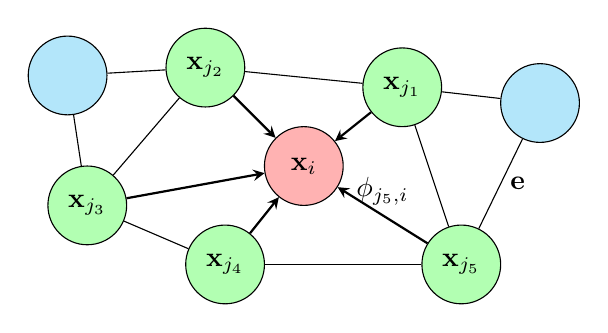
\begin{tikzpicture}[node distance=1.25cm]
        \node(main) [main_node] {$\mathbf{x}_i$};
        \node(neigh1) [neigh_node, right of=main, yshift=1cm] {$\mathbf{x}_{j_1}$};
        \node(neigh2) [neigh_node, left of=main, yshift=1.25cm] {$\mathbf{x}_{j_2}$};
        \node(neigh3) [neigh_node, left of=main, xshift=-1.5cm, yshift=-0.5cm] {$\mathbf{x}_{j_3}$};
        \node(neigh4) [neigh_node, below of=main, xshift=-1cm] {$\mathbf{x}_{j_4}$};
        \node(neigh5) [neigh_node, below of=main, xshift=2cm] {$\mathbf{x}_{j_5}$};

        \node(node1) [node, right of=neigh1, xshift=0.5cm, yshift=-0.2cm] {};
        \node(node2) [node, left of=neigh2, xshift=-0.5cm, yshift=-0.1cm] {};

        \draw[arrow] (neigh1) -- (main);
        \draw[arrow] (neigh2) -- (main);
        \draw[arrow] (neigh3) -- (main);
        \draw[arrow] (neigh4) -- (main);
        \draw[arrow] (neigh5) -- node[above]{$\phi_{j_5, i}$} (main);

        \draw (neigh1) -- (neigh2);
        \draw (neigh1) -- (neigh5);
        \draw (neigh2) -- (neigh3);
        \draw (neigh3) -- (neigh4);
        \draw (neigh4) -- (neigh5);
        \draw (neigh1) -- (node1);
        \draw (neigh5) -- node[right]{$\mathbf{e}$} (node1);
        \draw (neigh2) -- (node2);
        \draw (neigh3) -- (node2);
    \end{tikzpicture}
    \caption{Illustration of the message passing scheme}
\end{figure}

Different graph neural networks architecture can be constructed by specifying all this functions, in
particular the update function, since aggregation operation usually is chosen from the fixed list of
functions such as $\min$, $\max$, mean, sum, product, etc.

Also it is worth to point out, that the graph neural network has a property of locality: the next state of the node depends only on
the current state of the adjacent nodes (and incident edges if they exist), therefore the receptive field
of every node is limited to the number of layers or number of applying the layer to the given graph (usually
on each step different layers are applied).

\subsection{Minimum cost multicut problem}

The minimum cost multicut problem is a combinatorial problem which consists in binary
edge labeling for a given, not necessarily complete, weighted graph. The resulted labeling induced
a partitioning of the graph and can be recognized as an analogue of an instance segmentation for graphs and
that's why has a lot real-world application in computer vision and other fields.

\begin{definition}
    Let $G = (V, E, w)$ be a connected weighted graph, where $V$ is a set of nodes, $E$ -- set of edges and
    $w: E \to \mathbb{R}$ is a weight/cost function. Then the minimum cost multicut
    problem\footnote{The original paper has a typo in the definition of the problem}
    is the following:

    \begin{alignat*}{2}
        \min_{y \in \{0, 1\}^E} \quad &
        c(y) = \sum\limits_{e \in E} w_e y_e                                            \\
        \text{subject to:}      \quad &
        y_e \leq \sum\limits_{e' \in C \setminus \{e\}} y_{e'}                          \\
                                      & \forall C \in \text{cycles}(G), \forall e \in C
    \end{alignat*}
\end{definition}

The label $1$ means that the corresponding edge is cut.
And the cycle constraints ensure that if the edge was cut then there is no other path in the graph which connects
incident nodes of this edges.

This constraints can be reduced to only chordless cycles as it was shown by \citet{chopra1993partition}, but still for the
non complete graphs (where triangles inequality is sufficient) the constraints grows with size of graph exponentially, so can be
their enumeration can be practically infeasible.

From the point of view of hardness of this integer linear programming problem it is worth to mention that minimum cost multicut
is NP-hard.


\section{Problem statement}

\emph{State the problem addressed by the research article(s) rigorously, completely and concisely.
    You may deviate from the notation or terminology of the article(s) if this helps the reader to better connect its contents to preliminaries or related work.
    Do not motivate the problem.}

\section{Conceptual contributions}

\emph{In this main section of the report, state the conceptual (i.e.~non-empirical) contributions of the research article(s) completely, rigorously and in detail, using a consistent terminology and notation that may deviate from that of the article(s) if this helps the reader to better connect to preliminaries or related work.
    Prove all non-trivial statements and define all non-trivial algorithms in the form of pseudo-code.
    Fill in gaps the original article(s) leave to the reader (if any).
    Make additional figures if helpful, preferably using TikZ and PGF\footnote{\url{https://ctan.net/graphics/pgf/base/doc/pgfmanual.pdf}}.}

\section{Empirical contributions (if any, max.~1 column)}

\emph{State briefly the main empirical findings of the article(s) you are summarizing (if any).
    Do not copy or reproduce any figures or tables.}

\section{Ideas to improve the discussed approach}

\bibliography{../references.bib}
\bibliographystyle{plainnat}

\end{document}

